
%(BEGIN_QUESTION)
% Copyright 2010, Tony R. Kuphaldt, released under the Creative Commons Attribution License (v 1.0)
% This means you may do almost anything with this work of mine, so long as you give me proper credit

\noindent
{\bf Programming Challenge -- Mercury Cougar tail light sequencer}

\vskip 10pt

An instrument technician is restoring a vintage 1969 Mercury Cougar, which has three light bulbs on each side of the rear tail-light assembly for turn signals.  When the turn signal switch is activated, the three lights on that particular side of the car blink in sequence like this:

$$\includegraphics[width=15.5cm]{i03837x01.eps}$$

The problem is, the original factory sequencing circuit board for the tail lights is defective, so the technician decides to install a 12 VDC powered PLC in his Cougar to replicate the original blinking sequence.

\vskip 10pt

Write a PLC program to provide this blinking sequence with two switch inputs:

\begin{itemize}
\item{} Brake switch: if activated (and turn signal NOT activated) turn on all three lights constantly
\item{} Turn switch: when activated, blink the three lights in sequence regardless of brake switch status
\end{itemize}

\vskip 10pt

\vskip 20pt \vbox{\hrule \hbox{\strut \vrule{} {\bf Suggestions for Socratic discussion} \vrule} \hrule}

\begin{itemize}
\item{} Although a sequencing instruction is perhaps the most obvious way to perform this function, is there a way to sequence the tail lights {\it without} using a sequencing instruction?
\end{itemize}

\vfil

\noindent
PLC comparison:

\begin{itemize}
\item{} \underbar{Allen-Bradley Logix 5000}: relevant ladder-logic commands include {\tt SQI}, {\tt SQO}, and {\tt SQL}.
\vskip 5pt
\item{} \underbar{Allen-Bradley SLC 500}: relevant ladder-logic commands include {\tt SQI}, {\tt SQO}, {\tt SQC}, and {\tt SQL}. 
\vskip 5pt
\item{} \underbar{Siemens S7-200}: relevant ladder-logic commands include {\tt SCR}, {\tt SCRE}, and {\tt SCRT}.
\vskip 5pt
\item{} \underbar{Koyo (Automation Direct) DirectLogic}: relevant ladder-logic commands include {\tt DRUM} and {\tt EDRUM}.
\end{itemize}

\underbar{file i03837}
\eject
%(END_QUESTION)





%(BEGIN_ANSWER)


%(END_ANSWER)





%(BEGIN_NOTES)

I strongly recommend students save all their PLC programs for future reference, commenting them liberally and saving them with special filenames for easy searching at a later date!

\vskip 10pt

I also recommend presenting these programs as problems for students to work on in class for a short time period, then soliciting screenshot submissions from students (on flash drive, email, or some other electronic file transfer method) when that short time is up.  The purpose of this is to get students involved in PLC programming, and also to have them see other students' solutions to the same problem.  These screenshots may be emailed back to students at the conclusion of the day so they have other students' efforts to reference for further study.

%INDEX% PLC, programming challenge: Mercury Cougar tail light sequencer
%INDEX% Process: Mercury Cougar taillight blinker

%(END_NOTES)


